
\QCMautoevaluation{Pour chaque question, plusieurs réponses sont
  proposées.  Déterminer celles qui sont correctes.}

\begin{QCM}
  \begin{GroupeQCM}
    \begin{exercice}
      Sur quelle(s) figure(s) les points $A$ et $B$ sont‑ils symétriques par rapport à $d$ ?
      \begin{ChoixQCM}{4}
      \item 
      
      \includegraphics[width=1.8cm]{1_R1}
      \item 
      
      \includegraphics[width=1.8cm]{1_R2}
      \item 
      
      \includegraphics[width=1.8cm]{1_R3}
      \item 
      
      \includegraphics[width=1.8cm]{1_R4}
      \end{ChoixQCM}
\begin{corrige}
     \reponseQCM{cd} 
   \end{corrige}
    \end{exercice}
    
    
    \begin{exercice}
      \begin{center} 
\includegraphics[width=2.9cm]{Q2} \end{center}
      \begin{ChoixQCM}{4}
      \item $A$ et $K$ sont symétriques par rapport à $d$
      \item $C$ est le symétrique de $M$ par rapport à $d$
      \item $ABC$ et $KLM$ sont symétriques par rapport à $d$
      \item $KL = AB$
      \end{ChoixQCM}
\begin{corrige}
     \reponseQCM{ad}
   \end{corrige}
    \end{exercice}
    
    
    \begin{exercice}
      Dans quel(s) cas les triangles sont-ils symétriques par rapport à un axe ?
      \begin{ChoixQCM}{4}
      \item 
      
      \includegraphics[width=2.1cm]{3_R1}
      \item 
      
      
\includegraphics[width=2.1cm]{3_R2}
      \item 
      
      
\includegraphics[width=2.1cm]{3_R3}
      \item 
      
      \includegraphics[width=2.1cm]{3_R4}
      \end{ChoixQCM}
\begin{corrige}
     \reponseQCM{a}
   \end{corrige}
    \end{exercice}
    
    
    \end{GroupeQCM}
\end{QCM}
    
%%%%%%%%%%%%%%%%%%%%%%%%%%%%%%%%%%%
%%%%%%%%%%%%%%%%%%%%%%%%%%%%%%%%%%%
%MiseEnPage
%%%%%%%%%%%%%%%%%%%%%%%%%%%%%%%%%%%
\vfill
\newpage
%%%%%%%%%%%%%%%%%%%%%%%%%%%%%%%%%%%
%%%%%%%%%%%%%%%%%%%%%%%%%%%%%%%%%%%

    
    
\begin{QCM}
  \begin{GroupeQCM}

      \begin{exercice}
      \begin{center} 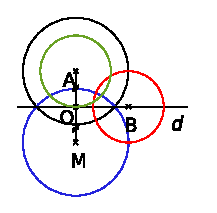
\includegraphics[width=3.1cm]{Q4} \end{center}
      \begin{ChoixQCM}{4}
      \item Les cercles noir et rouge sont symétriques par rapport à $d$
      \item Le cercle rouge est son propre symétrique par rapport à $d$
      \item Les cercles vert et rouge sont symétriques par rapport à $d$
      \item Les cercles bleu et noir sont symétriques par rapport à $d$
      \end{ChoixQCM}
\begin{corrige}
     \reponseQCM{bd}
   \end{corrige}
    \end{exercice}

  
  \begin{exercice}
      Sur quelle(s) figure(s) les points $A$ et $B$ sont‑ils symétriques par rapport à $O$ ?
      \begin{ChoixQCM}{4}
      \item 
      
      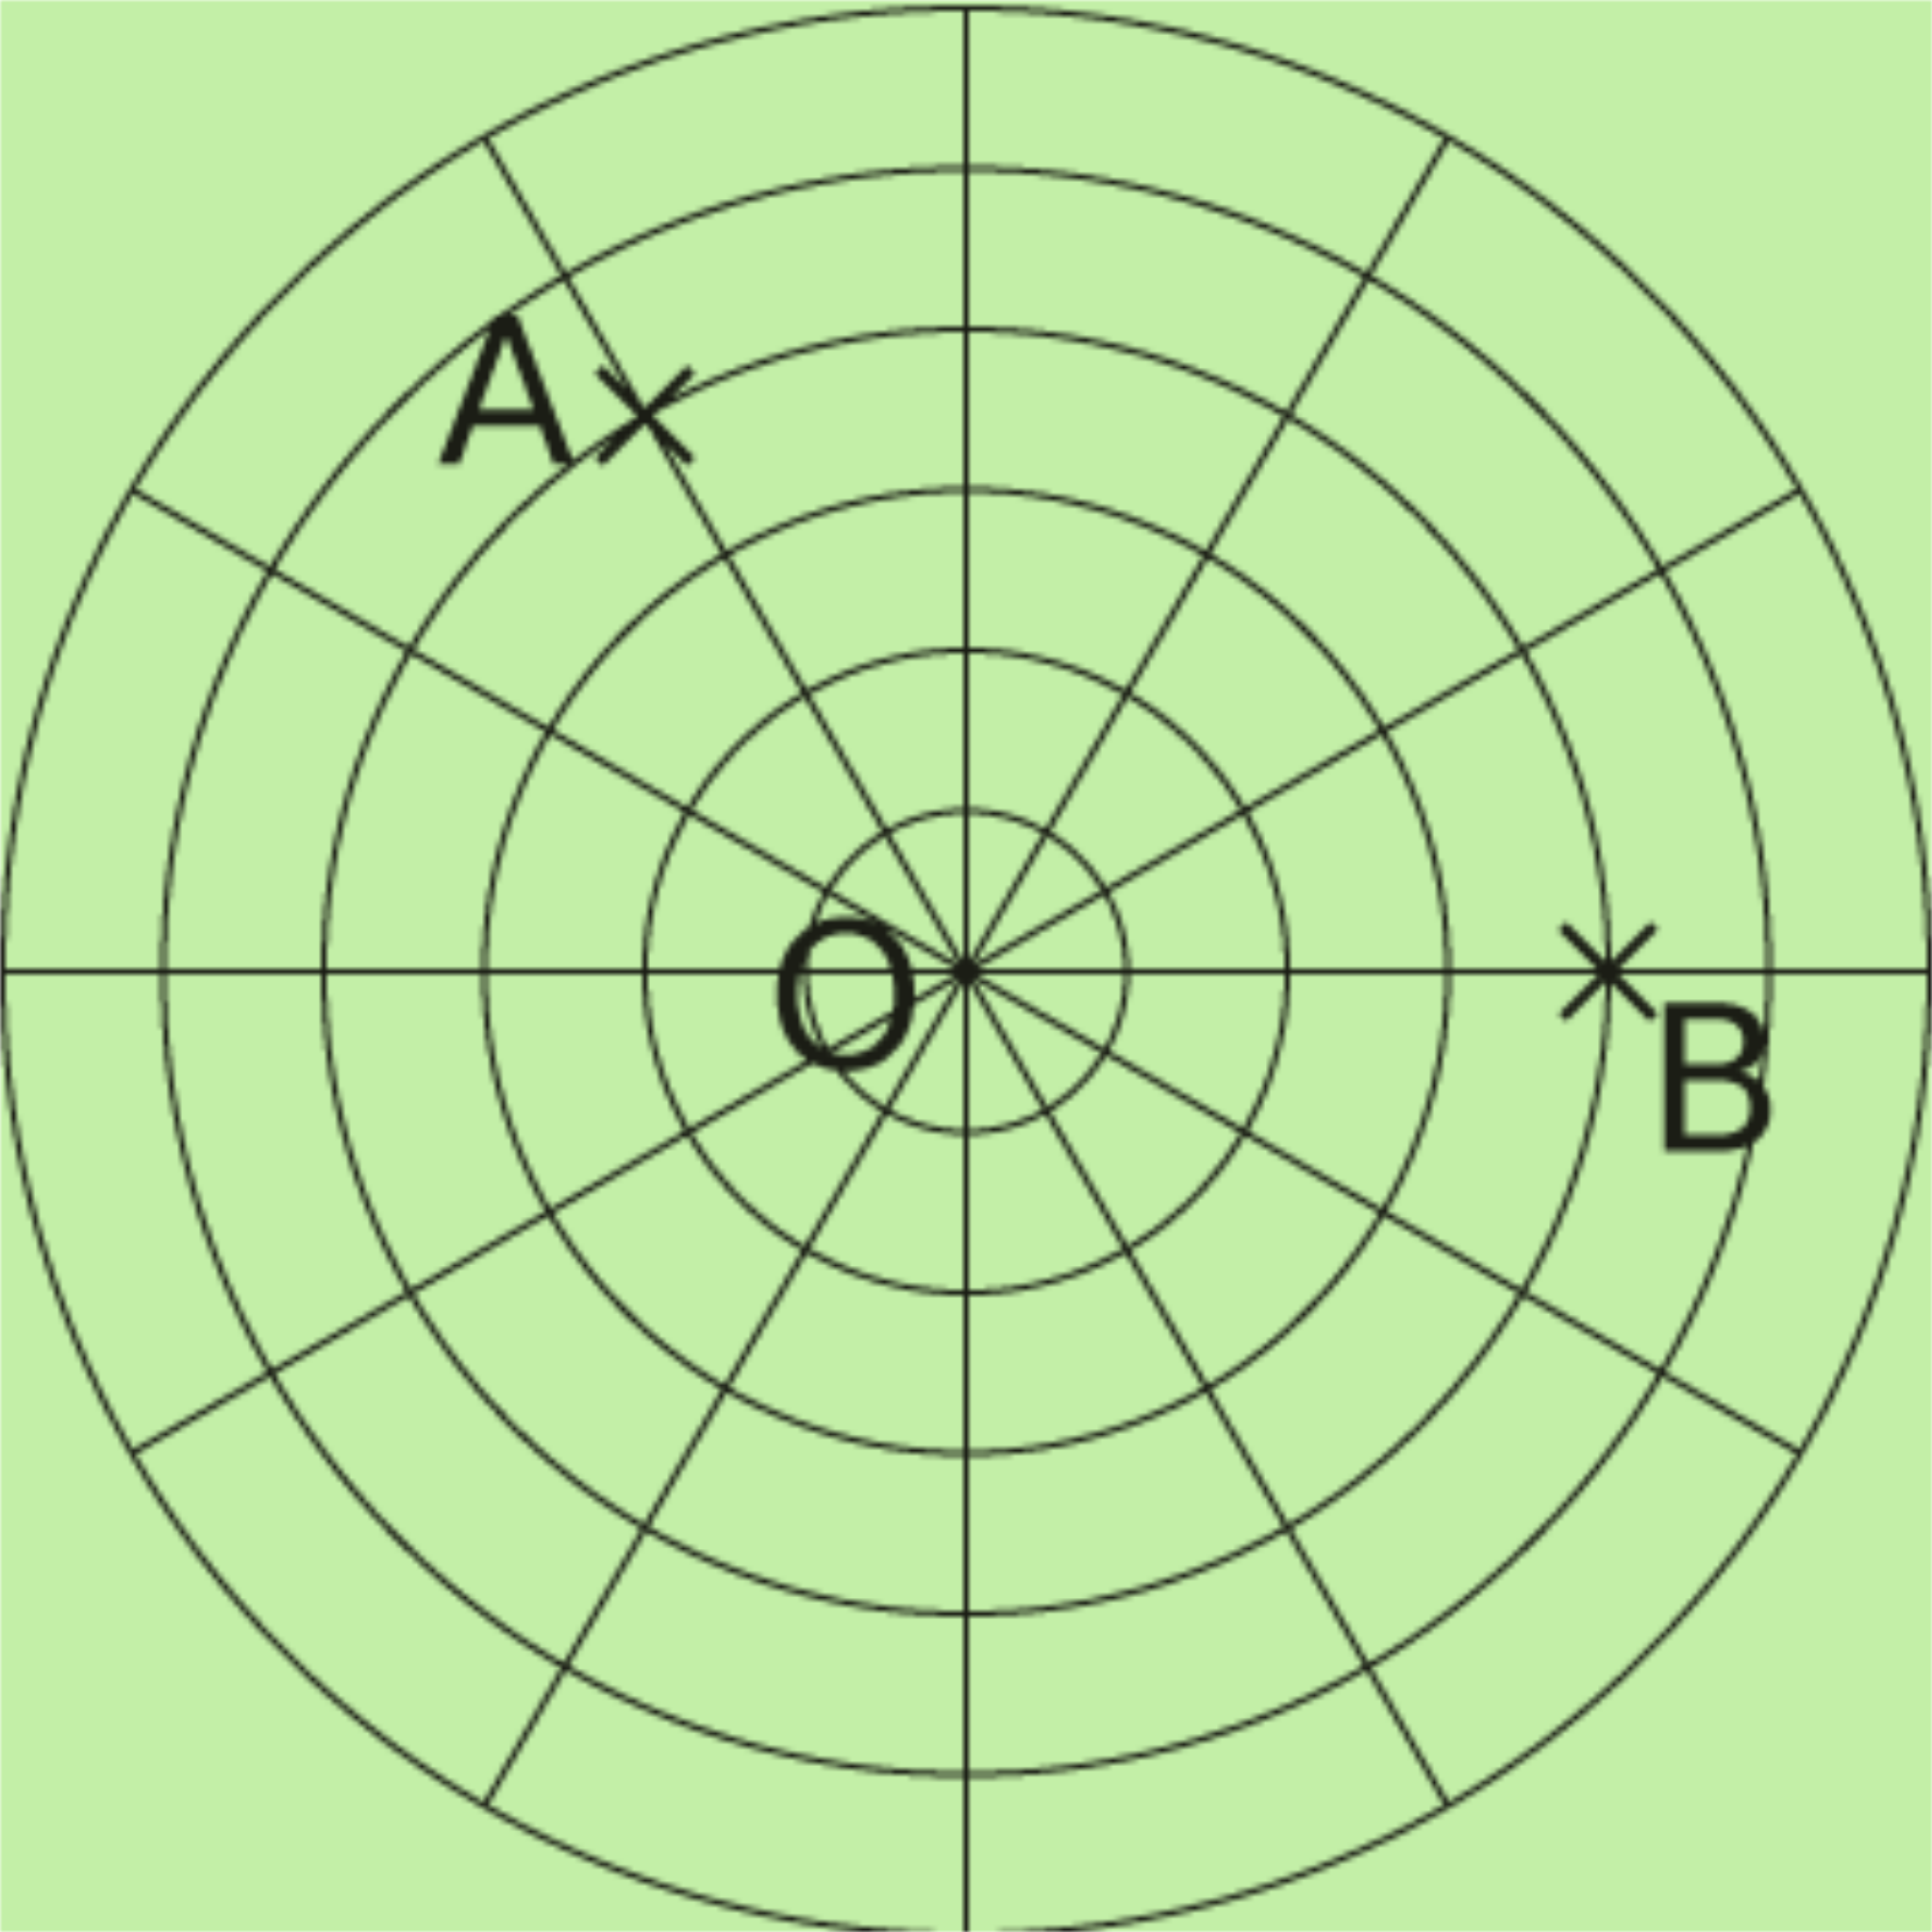
\includegraphics[width=2.7cm]{5_R1}
      \item 
      
      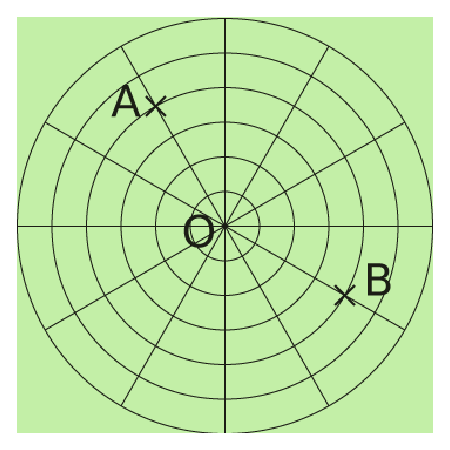
\includegraphics[width=2.7cm]{5_R2}
      \item 
      
      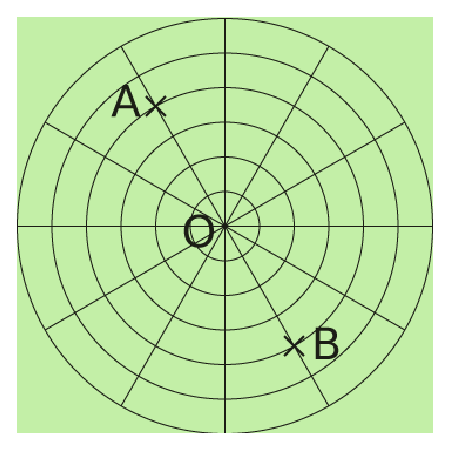
\includegraphics[width=2.7cm]{5_R3}
      \item 
      
      \includegraphics[width=2.7cm]{5_R4}
      \end{ChoixQCM}
\begin{corrige}
     \reponseQCM{c}
   \end{corrige}
    \end{exercice}
    
    
    \begin{exercice}
      Dans quel(s) cas les triangles sont-ils symétriques par rapport au centre $O$ ?
      \begin{ChoixQCM}{4}
      \item 
      
      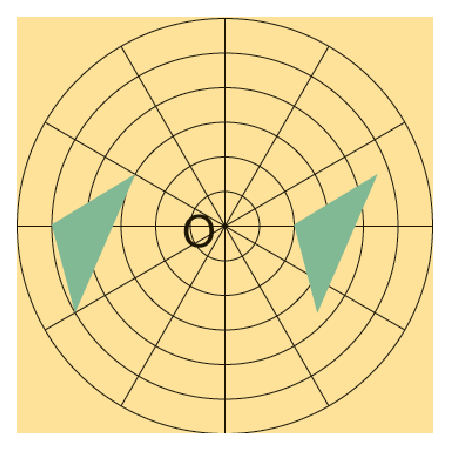
\includegraphics[width=2.7cm]{6_R1}
      \item 
      
      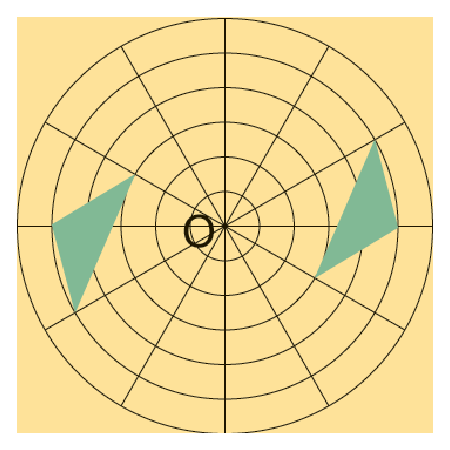
\includegraphics[width=2.7cm]{6_R2}
      \item 
      
      \includegraphics[width=2.7cm]{6_R3}
      \item 
      
      \includegraphics[width=2.7cm]{6_R4}
      \end{ChoixQCM}
\begin{corrige}
     \reponseQCM{b}
   \end{corrige}
    \end{exercice}
    \end{GroupeQCM}
\end{QCM}




  
